\documentclass[tikz, border=12pt]{standalone}
\usepackage{tikz}
\usepackage{xcolor}
\usetikzlibrary{arrows.meta, positioning, fit, backgrounds, calc}

%% Colors
\definecolor{ColAmber}{RGB}{204,133,0}
\definecolor{ColAmberDk}{RGB}{160,100,0}
\definecolor{ColGray}{RGB}{215,215,215}
\definecolor{ColGrayBd}{RGB}{90,90,90}
\definecolor{ColWhite}{RGB}{255,255,255}
\definecolor{ColDash}{RGB}{100,100,100}

%% Styles
\tikzset{
  box/.style={
    rectangle, draw=ColGrayBd, fill=ColWhite,
    minimum width=2.4cm, minimum height=0.8cm,
    align=center, font=\small
  },
  cat/.style={
    rectangle, draw=ColGrayBd, fill=ColGray,
    minimum width=2.4cm, minimum height=0.8cm,
    align=center, font=\small
  },
  proc/.style={
    rectangle, draw=ColAmberDk, fill=ColAmber,
    minimum width=2.6cm, minimum height=0.85cm,
    align=center, font=\small\bfseries, text=white
  },
  dregion/.style={
    rectangle, draw=ColDash, dashed,
    inner sep=6pt
  },
  op/.style={-Latex, draw=ColAmber, thick},
  exd/.style={-Latex, draw=black, dashed},
}

\begin{document}
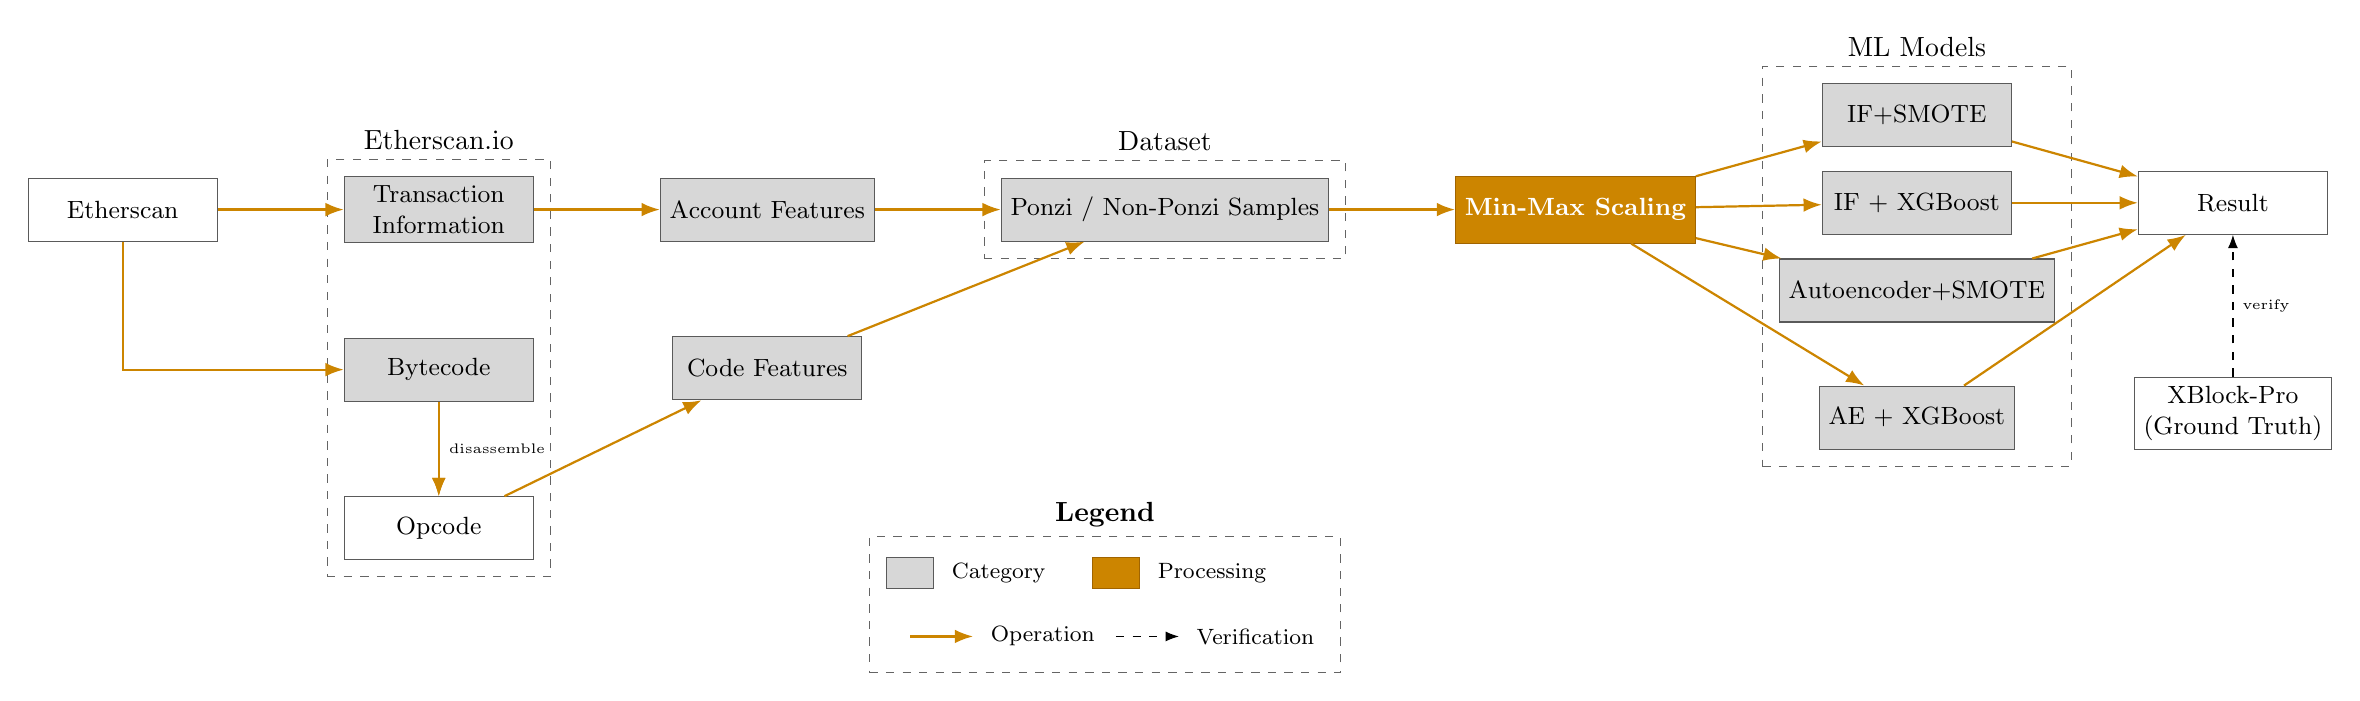
\begin{tikzpicture}[node distance=1.2cm and 1.6cm]

% ================= DATA =================
\node[box] (eth) {Etherscan};

% ================= RAW =================
\node[cat, right=of eth] (tx) {Transaction\\Information};
\node[cat, below=of tx] (byte) {Bytecode};
\node[box, below=of byte] (opcode) {Opcode};

\begin{scope}[on background layer]
\node[dregion, fit=(tx)(byte)(opcode), label=above:{Etherscan.io}] {};
\end{scope}

% ================= FEATURES =================
\node[cat, right=of tx] (acc) {Account Features};
\node[cat, below=of acc] (code) {Code Features};

% ================= DATASET =================
\node[cat, right=of acc] (dataset) {Ponzi / Non-Ponzi Samples};

\begin{scope}[on background layer]
\node[dregion, fit=(dataset), label=above:{Dataset}] {};
\end{scope}

% ================= PROCESS =================
\node[proc, right=of dataset] (scale) {Min-Max Scaling};

% ================= MODELS =================
\node[cat, right=of scale, yshift=1.2cm] (m1) {IF+SMOTE};
\node[cat, below=0.3cm of m1] (m2) {IF + XGBoost};
\node[cat, below=0.3cm of m2] (m3) {Autoencoder+SMOTE};
\node[cat, below=0.8cm of m3] (m4) {AE + XGBoost};

\begin{scope}[on background layer]
\node[dregion, fit=(m1)(m2)(m3)(m4), label=above:{ML Models}] {};
\end{scope}

% ================= RESULT =================
\node[box, right=of m2] (res) {Result};

% ================= GROUND TRUTH =================
\node[box, below=1.8cm of res] (xblock) {XBlock-Pro\\(Ground Truth)};

% ================= ARROWS =================
\draw[op] (eth) -- (tx);
\draw[op] (eth) |- (byte);

\draw[op] (tx) -- (acc);

\draw[op] (byte) -- (opcode);
\draw[op] (opcode) -- (code);
\draw[op] (byte.south) -- (opcode.north) node[midway, right] {\tiny disassemble};


\draw[op] (acc) -- (dataset);
\draw[op] (code) -- (dataset);

\draw[op] (dataset) -- (scale);

\draw[op] (scale) -- (m1);
\draw[op] (scale) -- (m2);
\draw[op] (scale) -- (m3);
\draw[op] (scale) -- (m4);

\draw[op] (m1) -- (res);
\draw[op] (m2) -- (res);
\draw[op] (m3) -- (res);
\draw[op] (m4) -- (res);

\draw[exd] (xblock.north) -- (res.south) node[midway, right] {\tiny verify};

% ================= LEGEND =================
\node[cat, minimum width=0.6cm, minimum height=0.4cm,
      below=4cm of eth, xshift=10cm] (Lcat) {};
\node[proc, minimum width=0.6cm, minimum height=0.4cm,
      right=2cm of Lcat] (Lproc) {};

% Labels
\node[right=0.1cm of Lcat] (tcat) {\footnotesize Category};
\node[right=0.1cm of Lproc] (tproc) {\footnotesize Processing};

% Operation arrow
\coordinate (a1) at ($(Lcat.south)+(0,-0.6)$);
\coordinate (a2) at ($(a1)+(0.8,0)$);
\draw[op] (a1) -- (a2);
\node[right=0.1cm of a2] (top) {\footnotesize Operation};

% Verification arrow
\coordinate (b1) at ($(Lproc.south)+(0,-0.6)$);
\coordinate (b2) at ($(b1)+(0.8,0)$);
\draw[exd] (b1) -- (b2);
\node[right=0.1cm of b2] (tver) {\footnotesize Verification};

% Legend box (FIXED)
\begin{scope}[on background layer]
\node[dregion,
      fit=(Lcat)(Lproc)(tcat)(tproc)(a1)(a2)(top)(b1)(b2)(tver),
      label=above:{\textbf{Legend}}] (legbox) {};
\end{scope}



\end{tikzpicture}
\end{document}